\label{subsec:exemplar_selection}

Exemplar selection is the process of selecting a subset of the training images along with
fiducial annotations that represent the range of variations in pose/expression/occlusion in the 
dataset. We term the set of images selected eventually as the \emph{exemplar set}. Ideally we would
like the exemplar set to be representative of the training set in that we would like to be able
to describe the pose/appearance of all images in the training set as some combinations of images
in the exemplar set, in a specific representation space. For example, given annotations of fiducial
locations in the training set, we would like have an exemplar set such that the shape of any training image
annotation (represented as an ordered list of pixel coordinates of various fiducial points) 
is a \emph{linear} combination of the annotations in the exemplar set.

\begin{figure}[!ht]
  \centering
  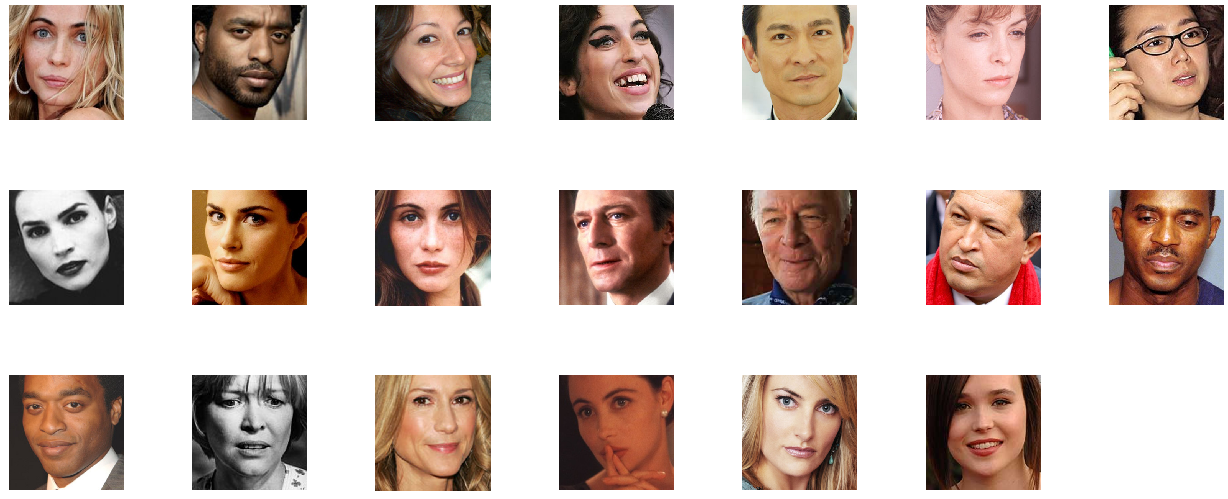
\includegraphics[width=15cm,height=6cm]{fid/figures/lfpw_exemplars_selected2.png}
  \caption{Examplars automatically selected by our clustering approach in
  Section~\ref{subsec:exemplar_selection} for LFPW dataset. Best viewed in color.}
  \label{fig:cofw_lfpw_exemplars}
\end{figure}
\begin{figure}[!ht]
  \centering
  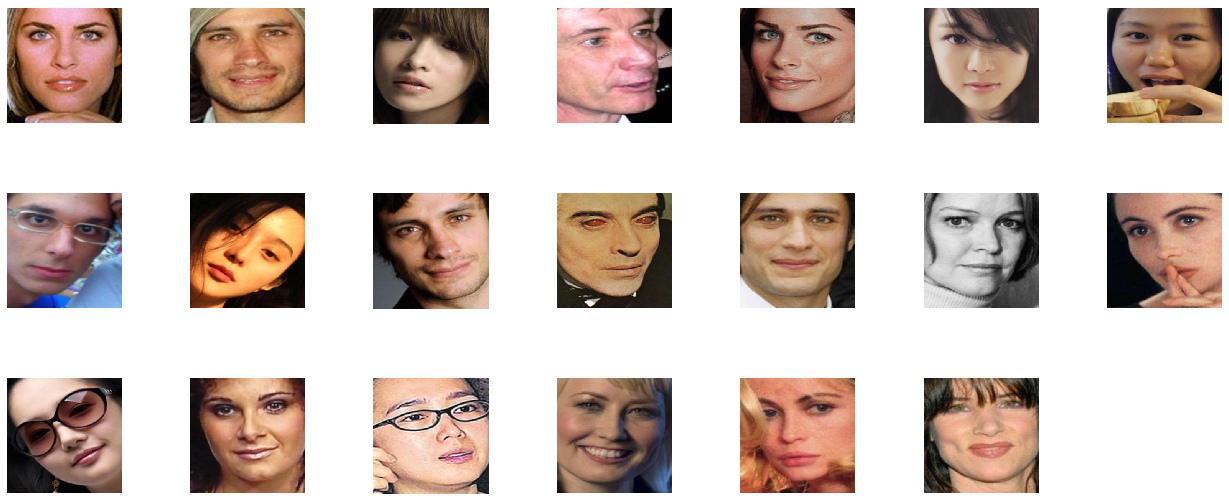
\includegraphics[width=15cm,height=6cm]{fid/figures/cofw_exemplars_selected2.png}
  \caption{Examplars automatically selected by our clustering approach in
  Section~\ref{subsec:exemplar_selection} for COFW dataset. Best viewed in color.}
  \label{fig:cofw_exemplars}
\end{figure}

Algorithm~\ref{alg:exemplar_selection} illustrates our basic exemplar selection algorithm.
The function \texttt{ComputeClusters} performs the operation of \texttt{kmeans} clustering in the
vector space of fiducials, or feature vectors depending upon its input arguments.
While the algorithm outputs two datasets for shape based and appearance based exemplars, note
that shape based exemplars can be further divided into pose and expression classes and
appearance based exemplars can also be tuned to include some examples of occlusion.
However, we found that \texttt{kmeans} inadvertently does this since it clusters fiducials
of the same pose but varying expression (shape clustering) or occlusion (appearance
clustering) into one cluster.
